\documentclass[a4paper,10pt]{article}

\usepackage[utf8]{inputenc}
\usepackage[T1]{fontenc}
\usepackage[spanish]{babel}
\usepackage{fullpage}
\usepackage{csquotes}
\usepackage[backend=biber,style=numeric,sorting=ynt]{biblatex}
\usepackage{xcolor}
\usepackage{hyperref}
\usepackage{sepfootnotes}
\usepackage{tikz}
\usepackage{pgf-umlsd}
\usepackage{graphicx}

\newcommand{\borrador}[1]{{\color{red}{#1}}}
\newcommand\nombre{\textsc}
\newcommand{\codigo}{\texttt}
\newcommand{\runner}{\textit{Runner}}
\newcommand{\pyGob}{\nombre{PyGobstones}}

\addbibresource{main.bib}

\setlength\parindent{1em}

\title{Implementación de un runner de Gobstones para la plataforma Mumuki}
\author{Federico Aloi}

\begin{document}

\maketitle

%!TEX root = main.tex

\newcommand{\caracteristica}[1]{\item \textbf{#1:}}

\section{Introducción}
La informática ha tenido sus inicios entre matemáticos (como Alan Turing\footnote{Turing} y John von Neumann\footnote{VonNeumann}) y, algunas décadas después, con la invención del circuito integrado, los electrónicos. Debido a las limitaciones tecnológicas de aquellas primeras computadoras, es razonable que la primera percepción de programación estuviera fuertemente acoplada a la máquina, ya que resultaba imposible pensar una cosa sin la otra. Como ejemplo de esto, basta mencionar la conocida anécdota del \textit{bug}\footnote{Bug}, que persiste hoy en día como metáfora asociada a una falla dentro de un programa.
\\\\
\borrador{
Mini mini reseña de cómo se fue pasando del bajo al alto nivel, y cómo esto era necesario porque el hardware no daba para más.
}
\\\\
Esta manera de percibir a la programación puede verse reflejada en muchos cursos iniciales, donde se hace énfasis en cuestiones que tienen más que ver con el \textit{hardware} subyacente que con el \textit{software} que se pretende construir: se favorece a la performance del programa por sobre otros atributos como expresividad, abstracción, declaratividad. Si bien este enfoque es válido en ciertos contextos, en muchos otros (y sobre todo en un primer acercamiento a la programación) no sólo que no aportan sino que muchas veces lo único que se logra es ahuyentar a los estudiantes, transmitiendo que la programación es un arte oscuro e incomprensible, exclusivo para unos pocos.
\\\\
En contraposición a este enfoque, surge una nueva forma de enseñar a programar que pretende ser más inclusiva y más didáctica, haciendo uso intensivo de herramientas tecnológicas para asistir al docente en su rol de educador. Algunas herramientas que han ido surgiendo en los últimos años son: Logo, Alice, Scratch, y más recientemente Pilas Bloques, Wollok, Gobstones y Mumuki. \borrador{citar o explicar qué son todas esas cosas que nombré}.
\\\\
Si bien cada una de esas herramientas es diferente, podemos identificar ciertas características compartidas:
\begin{itemize}
  \caracteristica{componentes visuales}
  \caracteristica{pensadas para el ámbito educativo}
  \caracteristica{requieren un trabajo fuerte por parte del docente}
  \caracteristica{esconden aspectos netamente tecnológicos}
\end{itemize}

De las herramientas mencionadas, el presente trabajo se concentrará en Gobstones y Mumuki, considerando que pueden complementarse muy bien, logrando así enriquecer aún más el método de enseñanza de un curso introductorio en programación. Veremos a continuación de qué se ocupa cada uno de estos proyectos.

\subsection{Gobstones, una nueva forma de aprender a programar}
El proyecto Gobstones consta de dos componentes fundamentales: una secuencia didáctica y un lenguaje de programación que permite ponerla en práctica.
\\\\
Según el Dr. Martínez López, fundador del proyecto, ``esta secuencia didáctica novedosa, diferente a la tradicional forma de enseñar programación, se diseñó teniendo en cuenta el trabajo con los estudiantes de primer año de la Tecnicatura en Programación Informática (TPI) de la Universidad Nacional de Quilmes, y expresa una síntesis conceptual utilizable con personas que no tienen ninguna experiencia previa en programación, ni demasiada familiaridad con procesos de abstracción.''\cite{LibroGobstones}. La secuencia favorece la abstracción desde el primer momento, prestando especial atención al uso de procedimientos y funciones y postergando otros conceptos como la repetición condicional o el uso de variables hasta el momento en que realmente surge la necesidad de utilizarlos.
\\\\
En cuanto al lenguaje, escribe que ``Gobstones es un lenguaje conciso de sintaxis razonablemente simple, orientado a personas que no tienen conocimientos previos en programación. El lenguaje maneja distintos componentes propios, ideados con el fin de aprender a resolver problemas en programación, pero al mismo tiempo intentando volver atractivo el aprendizaje, para lograr captar la atención y capacidad de asombro del estudiante.''\cite{LibroGobstones}. No es posible realizar operaciones de entrada/salida tradicionales como la impresión por pantalla o la lectoescritura de archivos, el único contacto con el ``mundo exterior'' se da a través de un tablero de dimensiones configurables, que puede contener infinitas bolitas de colores en cada una de sus celdas y además cuenta con un cabezal que permite desplazarse por el mismo.
\\\\
Además de ser utilizado en la materia Introducción a la Programación de la Tecnicatura antes mencionada, Gobstones se utiliza actualmente en la Escuela Fiorentino Ameghino de Florencio Varela y en el Instituto Sagrado Corazón Al.Cal. de Villa Jardín.
\\\\
Tanto la escritura de programas como su ejecución ocurren dentro de la herramienta \nombre{PyGobstones}\footnote{Puede descargarse desde \url{http://www.gobstones.org/?page_id=30}}, desarrollada por el Lic. Pablo Barenbaum en conjunto con estudiantes de TPI. Al momento de escribir este trabajo, existe un equipo encargado de mantener el software, liderado por el Lic. Ary Batista, al cual he acudido en diferentes instancias durante el desarrollo para evacuar dudas sobre el funcionamiento, reportar errores y solicitar algunas extensiones.

\subsection{Mumuki, educación libre de la programación}
Mumuki es un proyecto que apunta a universalizar el acceso a la educación libre, gratuita y de calidad; enfocándose principal pero no excluyentemente en la enseñanza de la programación. Según sus fundadores es, además, ``un software educativo para aprender a programar a partir de la resolución de problemas; plantea enseñar conceptos de programación, en un proceso conducido por guías prácticas en las que la teoría surge a medida que se avanza. Esta herramienta se presenta al estudiante como una aplicación Web interactiva, en la que se articulan explicaciones y ejemplos con la opción de que cada uno realice su propia solución y la plataforma la pruebe y corrija instantáneamente, orientando acerca de los aciertos y errores. Está diseñado para ser utilizado tanto a distancia, como recurso complementario al aula y con el ritmo propio que cada estudiante le imprime a su forma de practicar, como en espacios educativos formales de laboratorios o talleres, donde cada alumno -o grupo- trabaja con su máquina, con la presencia orientadora de los docentes.''\cite{PaperMumuki}
\\\\
Está compuesto por las siguientes herramientas:
\begin{itemize}
  \caracteristica{la plataforma web} el entorno donde los estudiantes resuelven los ejercicios de programación y ven el \textit{feedback} generado por la herramienta. Cada estudiante tiene su propia cuenta de usuario y puede ver en todo momento su progreso y las soluciones que envió
  \caracteristica{los \textit{runners}} servicios web que se encargan de compilar, ejecutar y probar los programas enviados por los estudiantes
  \caracteristica{Classroom} herramienta pensada para realizar el seguimiento de los estudiantes, diseñada para ser utilizada tanto dentro como fuera del aula
  \caracteristica{Bibliotheca} repositorio de guías y ejercicios, públicamente accesible y con posibilidad de crear ejercicios completamente nuevos o adaptar alguno existente para cumplir con necesidades particulares
\end{itemize}

Existe una notable comunidad de desarrolladores involucrada en el proyecto, liderados por el Ing. Franco Bulgarelli. A partir de la realización de la extensión que explicaré más adelante, me involucré activamente en el equipo del proyecto, del cual también soy responsable hoy en día.
\\\\
Al día de hoy, la suite de herramientas está siendo utilizada en varias universidades: Universidad Tecnológica Nacional, Universidad Nacional de Quilmes y Universidad Nacional de Avellaneda; y en un colegio secundario, el Instituto Sagrado Corazón Al.Cal. de Villa Jardín.

\subsection{Problema}

%!TEX root = main.tex

\section{Requerimientos}
En esta sección veremos cómo funcionan las herramientas involucradas y cuáles son los puntos de extensión que proveen.

\subsection{Arquitectura de Mumuki}
Antes de empezar a hablar de la arquitectura, es necesario entender cómo se estructura el contenido dentro de la plataforma, ya que esto impacta en cada uno de los componentes.

El ejercicio es la mínima unidad de contenido: se trata de una descripción de un problema y una forma de evaluarlo. Desde el punto de vista del estudiante, consta de un título, una descripción del problema, una serie de ayudas adicionales y un corolario (que se muestra tras resolver el problema correctamente). Desde el punto de vista técnico, se estructura de la siguiente manera:

\begin{itemize}
  \caracteristica{Pruebas} evalúan que la solución resuelva el problema de forma correcta, es decir, que llegue al resultado esperado.

  Por ejemplo, si tenemos una función \codigo{dobleDe(numero)} que recibe un número y devuelve su doble, una prueba posible sería que \codigo{dobleDe(2)} da como resultado \codigo{4}.

  \caracteristica{Expectativas} evalúan que la solución resuelva el problema de forma adecuada, es decir, que se utilicen las herramientas correctas.

  Supongamos que ahora queremos hacer la función \codigo{cuadrupleDe(numero)}, que tome un número y devuelve su cuadruple, y queremos que el estudiante la implemente en términos de \codigo{dobleDe} (ya que multiplicar por 4 es lo mismo que multiplicar 2 veces por 2). En ese caso nuestro objetivo sería \codigo{cuadrupleDe(numero) \textit{debe usar} dobleDe(numero)}.

  \caracteristica{Código adicional} herramientas que el estudiante puede utilizar al escribir su solución. Pueden ser fruto de ejercicios anteriores o simplemente partes del problema que el docente quiera facilitar.

  Retomando el ejemplo anterior, la función \codigo{dobleDe(numero)} podría ser provista por el docente, ya que se supone que el estudiante pudo razonarla en el ejercicio anterior y sería tedioso que tuviera que volver a escribirla.
\end{itemize}

De los componentes mencionados en la introducción, sólo nos interesan el Atheneum y los \runner s ya que como vemos en la Figura \ref{fig:FlujoSubmission} son los que intervienen en el proceso que va desde el envío de la solución del estudiante hasta la obtención del resultado.

A grandes rasgos, la comunicación se realiza de la siguiente manera:
\begin{itemize}
  \item{El estudiante envia su solución, lo cual produce un POST HTTP hacia el Atheneum.}
  \item{El Atheneum envia otro POST HTTP al \runner\ correspondiente, agregando las pruebas, expectativas y código adicional del ejercicio.}
  \item{El \runner\ responde al pedido HTTP con el resultado de evaluar la solución, que puede ser: \codigo{errored} si el programa no compila, \codigo{passed\_with\_warnings} si el programa es correcto (pasa las pruebas) pero no utiliza las herramientas adecuadas o \codigo{passed} si es correcto y cumple con las expectativas.}
\end{itemize}

\begin{figure}
  \centering

  \begin{sequencediagram}
    \newthread{estudiante}{Estudiante}{}
    \newinst{atheneum}{Atheneum}{}
    \newinst{runner}{Runner}{}

    \begin{call}{estudiante}{Validar(solucion)}{atheneum}{resultado}
      \begin{call}{atheneum}{Validar(solucion, pruebas, expectativas, codigo\_adicional)}{runner}{resultado}
      \end{call}
    \end{call}
  \end{sequencediagram}

  \caption{Comunicación entre el estudiante, el Atheneum y un \runner.}
  \label{fig:FlujoSubmission}
\end{figure}

\subsection{Requisitos para poder implementar un \runner}
Para poder implementar un \runner, es necesario que el lenguaje cumpla ciertas características.

\sepfootnotecontent
  {GBB}
  {Acrónimo para GoBstones Board. Es un archivo de texto plano con un formato particular que permite especificar tableros.}

La primera de ellas: tiene que poderse ejecutar por línea de comandos, sin la intervención de un humano. Si bien esto puede sonar trivial cuando de lenguajes industriales se trata, no lo es para este tipo de herramientas didácticas. Suelen estar fuertemente acopladas con el entorno visual que proveen para programar, haciendo que no sea posible ejecutar fuera de allí (lo que imposibilita, por ejemplo, crear un \runner\ que ejecute un programa hecho en Scratch). Afortunadamente \pyGob\ sí cuenta con dicha posibilidad, pueden ejecutarse programas por la consola y visualizar el resultado en formato GBB\sepfootnote{GBB} o HTML.

Lo siguiente es poder probar que la solución del estudiante sea correcta. De un programa Gobstones pueden interesarnos validar dos cosas: dado un tablero inicial conocido, el problema tiene que llegar a un tablero final esperado (si se trata de un procedimiento) o tiene que retornar un valor esperado (si se trata de una función). Este tipo de pruebas se denominan unitarias y suelen ser escritas en algún framework específico del lenguaje con el que se está trabajando: JUnit para Java, rspec para Ruby, mocha para Javascript,etcétera. En este caso tuve que desarrollarlo yo, ya que hasta el momento no existía un framework así para Gobstones.

\sepfootnotecontent
  {AST}
  {Representación de árbol de la estructura sintáctica abstracta (simplificada) del código fuente, donde cada nodo del árbol denota una construcción que ocurre en el código fuente. La sintaxis es abstracta en el sentido que no representa cada detalle que aparezca en la sintaxis verdadera, omitiendo, por ejemplo, comentarios, espacios y saltos de línea.}

Por último, se tiene que poder analizar el código del estudiante para verificar si se cumplen las expectativas. La forma más sencilla de lograrlo es recorriendo el árbol de sintaxis abstracta (AST\sepfootnote{AST}), buscando que existan ciertos patrones. Si bien \pyGob\ ya proveía una manera de obtener el AST, tuve que solicitarle al equipo de desarrollo algunos cambios que comentaré más adelante.

\subsection{Cambios realizados en \pyGob}
\sepfootnotecontent
  {Abalorios}
  {En paralelo al desarrollo de este trabajo y sin saber de la existencia del mismo, surgió una iniciativa similar por parte del Lic. Pablo Barenbaum, docente de la cátedra Introducción a la Programación en UNQ. Al enterarnos de que estabamos trabajando en proyectos similares, se optó por pausar el desarrollo de Abalorios.}

\sepfootnotecontent
  {PullRequestHTML}
  {Pueden verse los cambios realizados en \url{https://github.com/gobstones/PyGobstones-Lang/pull/1}.}

La visualización HTML del tablero que proveía el intérprete era poco atractiva y distaba mucho de la identidad visual de Gobstones. Basado en la representación que el Lic. Pablo Barenbaum confeccionó para la herramienta Abalorios\sepfootnote{Abalorios}, creé una nueva representación (ver Figura \ref{fig:TableroHTML}) que luego fue integrada a la versión estable de \pyGob\sepfootnote{PullRequestHTML}.

\begin{figure}
  \centering
  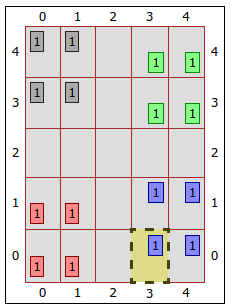
\includegraphics[scale=0.5]{images/tablero-html-viejo.png}
  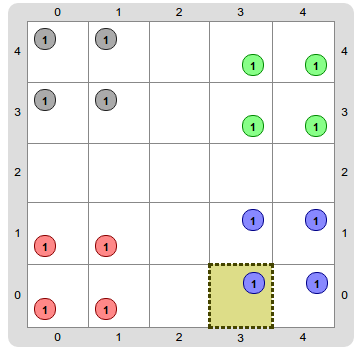
\includegraphics[scale=0.4]{images/tablero-html-nuevo.png}

  \caption{Representación HTML de un tablero. La versión de la izquierda era la existente hasta la realización del presente trabajo.}
  \label{fig:TableroHTML}
\end{figure}

\sepfootnotecontent
  {IssueAST}
  {Puede verse la discusión en \url{https://github.com/gobstones/PyGobstones/issues/32}.}

Con la generación del AST ocurrieron dos problemas puntuales, que fueron resueltos por el equipo desarrollador al poco tiempo de haberlos reportado\sepfootnote{IssueAST}.

El primero fue que además de generarse el AST se ejecutaba el código, inhabilitando la posibilidad de correr expectativas sobre programas sintácticamente válidos que arrojaban error en tiempo de ejecución. El siguiente problema fue que no era posible generar el AST de una única función o procedimiento, lo cual obligaba a tener que correr las expectativas sobre el código del estudiante y el provisto por el docente, sin poder diferenciar fácilmente qué parte se estaba analizando.

%!TEX root = main.tex

\section{Implementación}

\subsection{Tecnología elegida}
Al pensar cuál podría ser la tecnología más adecuada para desarrollar el \runner, lo primero que surge es evaluar con qué tecnologías fueron construidos los \runner s existentes y cuánto de ello podría ser reutilizado.

\sepfootnotecontent
  {Gema}
  {Nombre con el que se conoce a las bibliotecas de código Ruby. Tienen la particularidad de ser muy fáciles de publicar y usar, favoreciendo así la reutilización de componentes.}

En el momento en que empecé a planificar la integración, Mumuki soportaba solamente 3 lenguajes: Haskell, con un \runner\ escrito en Haskell, y Prolog y Ruby, ambos con \runner s escritos en Ruby. Estos dos últimos compartían parte de su código mediante la utilización de la gema\sepfootnote{Gema} \mumukit, encargada de resolver las cuestiones de comunicación con el Atheneum, dejando como tarea para el programador la implementación de algunos pocos métodos que se encargan de lo necesario para ejecutar los programas.

Ante este escenario, resulta evidente que la elección de Ruby como lenguaje de soporte para el \runner\ de Gobstones era la más acertada.

\subsection{Stones Spec}
Una vez elegida la tecnología, me aboqué a la primera tarea: crear un framework para poder correr tests unitarios sobre programas, procedimientos o funciones Gobstones. En cualquier lenguaje de propósito general, estos frameworks están codificados utilizando el mismo lenguaje sobre el cual se van a ejecutar las pruebas pero como Gobstones no es un lenguaje de propósito general, esto no era una opción. Por simplicidad y para no introducir otro nuevo lenguaje, elegí utilizar también Ruby para esta tarea.

Tras analizar algunos ejercicios de las guías de Introducción a la Programación, diseñé un modelo de prueba que consta de los siguientes atributos:

\begin{itemize}
  \caracteristica{Subject} nombre del procedimiento o función que se desea probar. Si se lo omite, las pruebas se realizan sobre el programa completo.
  \caracteristica{Check head position} indica si las pruebas deben verificar la posición del cabezal.
  \caracteristica{Examples} lista de ejemplos que serán probados, la estructura dependerá del sujeto que se esté probando.

  En el caso de un \emph{programa}, cada ejemplo constará de una dupla \codigo{(tablero inicial, tablero final)} (ver código \ref{lst:ProgramSpec}); para un \emph{procedimiento} con parámetros, deberán especificarse también los parámetros con los cuales será ejecutado, resultando en una terna \codigo{(parámetros, tablero inicial, tablero final)} (ver código \ref{lst:ProcedureSpec}); y para una \emph{función} deberá especificarse el resultado esperado en vez del tablero final, resultando en una terna \codigo{(parámetros, tablero inicial, resultado)} (ver código \ref{lst:FunctionSpec}).
\end{itemize}

\begin{listing}
  \centering

  \begin{minted}{yaml}
  check_head_position: true
  examples:
   - initial_board: |
       GBB/1.0
       size 2 2
       head 0 0
     final_board: |
       GBB/1.0
       cell 1 1 Rojo 1
       size 2 2
       head 1 1
  \end{minted}

  \caption{Ejemplo de un test de \emph{programa}, que chequea que haya una bolita roja en la celda \codigo{(1, 1)} y que el cabezal se encuentre allí.}
  \label{lst:ProgramSpec}
\end{listing}

\begin{listing}
  \centering

  \begin{minted}{yaml}
  subject: PonerN
  examples:
   - arguments:
      - 2
      - Azul
     initial_board: |
       GBB/1.0
       size 2 2
       head 0 0
     final_board: |
       GBB/1.0
       size 2 2
       cell 0 0 Azul 2
       head 0 0
  \end{minted}

  \caption{Ejemplo de un test de \emph{procedimiento}, que chequea que \codigo{PonerN} pone 2 bolitas azules cuando es llamado con los argumentos \codigo{(2, Azul)}.}
  \label{lst:ProcedureSpec}
\end{listing}

\begin{listing}
  \centering

  \begin{minted}{yaml}
  subject: nroBolitasTotal
  examples:
   - initial_board: |
       GBB/1.0
       size 2 2
       cell 0 0 Rojo 1 Azul 2 Negro 2 Verde 5
       head 0 0
     return: 10
  \end{minted}

  \caption{Ejemplo de un test de \emph{función}, que chequea que \codigo{nroBolitasTotal} devuelve 10 en una celda con 10 bolitas.}
  \label{lst:FunctionSpec}
\end{listing}

\borrador{Contar brevemente cómo se implementó: se crean archivos temporales con el programa y los tableros iniciales, se ejecuta, se parsea el resultado de la consola o del archivo GBB de salida.}

\subsection{Trabajando con \mumukit}
En particular, \mumukit\ exige que se implementen al menos dos métodos:
\begin{itemize}
  \item{\codigo{compile}: que recibe la solución del estudiante, el código extra provisto por el docente y el código de las pruebas, y debe encargarse de unirlos;}
  \item{\codigo{run\_test\_command}: que recibe el archivo generado por el método anterior y debe encargarse de ejecutar las pruebas y devolver el resultado.}
\end{itemize}

En cualquier otro \runner, programar el \codigo{compile} es muy sencillo: como todos los bloques de código están expresados en el lenguaje que se intenta probar, basta con yuxtaponerlos. Como vimos anteriormente, un test unitario en Gobstones no es un archivo de código sino una representación YAML de una serie de configuraciones, y eso es lo que se genera en este caso.

\subsection{Extensiones a Mumuki}
\borrador{
  \begin{itemize}
    \item poder mostrar el resultado de una ejecución, para no perder el componente visual de Gobstones. Hasta el momento no existía ya que en otros lenguajes no interesaba mostrar el resultado
    \item soportar HTML como output de un runner
  \end{itemize}
}

\subsection{Mumuki Gobstones Server}
\subsubsection{Integración con Stones Spec}
\subsubsection{Chequeo de expectativas}

%!TEX root = main.tex

\section{Pruebas}
\subsection{Testing automatizado del código}
\borrador{
  Porcentaje de cobertura, tipos de tests que existen.
}

\subsection{Utilización de las herramientas en un colegio secundario}
\borrador{
  \begin{itemize}
    \item background de la escuela
    \item cómo se utilizó la herramienta
    \item aceptación por parte de los estudiantes
    \item quizás disparar una encuesta? ojo, queda poco tiempo y a la mayoría de los pibes ya no los veo
  \end{itemize}
}

\subsection{Prueba de concepto listas en XGobstones en UNQ Belgrano}
\borrador{
  \begin{itemize}
    \item background de los estudiantes
    \item cómo se utilizó la herramienta
    \item aceptación por parte de los estudiantes
    \item quizás disparar una encuesta?
  \end{itemize}
}

%!TEX root = main.tex

\section{Trabajo futuro}

\subsubsection{Integración con Gobstones Web}
Está siendo desarrollada una nueva versión de Gobstones basada en Javascript, que estará disponible para ser utilizada desde la web y reemplazará a \pyGob. Cuando eso suceda, parte de la integración que se realizó en el presente trabajo quedará obsoleta y será conveniente volver a desarrollarla.

A pesar de esto, tener una versión web de Gobstones presenta algunas ventajas: la ejecución y la generación del AST podrían realizarse directamente en el servidor de Gobstones, componentes como la visualización HTML del tablero o el editor podrían ser reutilizados por ambos proyectos, etc. Podría también desarrollarse una integración mucho más fuerte, proveyendo al estudiante de ejercicios directamente sobre el IDE que utiliza día a día, sin necesidad de que este tenga que resolver ejercicios en dos lugares diferentes.

\subsubsection{Motor de expectativas}
Dentro de las tareas planificadas dentro del proyecto Mumuki está la de crear un motor de expectativas que permita reutilizar gran parte del código que hoy está replicado en cada uno de los \runner s, ya que los patrones que se quieren chequear suelen ser similares entre lenguajes con características similares (por ejemplo, las inspecciones \codigo{HasBinding} y \codigo{HasUsage} resultan útiles para cualquier lenguaje, y las implementaciones son prácticamente iguales).

Una vez que dicha herramienta exista, habrá que convertir el AST de Gobstones al formato que esta espere y traducir las expectativas existentes a Haskell, tecnología en la cual será construido el motor. Esto permitirá aumentar notablemente la cantidad de expectativas soportadas por el \runner\ de Gobstones, ya que podrán utilizarse todas las que ya existan para otros lenguajes.

\subsubsection{Soporte completo para XGobstones}
Para que la herramienta pueda ser utilizada durante todo un curso de Introducción a la Programación, es necesario incorporar soporte para XGobstones, extensión que agrega listas y registros al lenguaje.

Actualmente existe una prueba de concepto que realicé para dar soporte a una guía de recorridos sobre listas que fue utilizada en el curso dictado el segundo semestre de 2015 en el CIU General Belgrano. Dicha prueba permitió especificar pruebas sobre funciones de manipulación de listas que no hacían uso del tablero, pudiendo verificar que devolvían la lista esperada.

Para seguir con esta línea, habría que implementar más tipos de aserciones sobre listas, como por ejemplo saber su longitud o aceptar cualquier permutación como resultado válido, e incorporar aserciones que permitan validar registros.

%!TEX root = main.tex

\section{Conclusiones}
Si bien todavía faltan funcionalidades para considerar que la integración con Gobstones está completa, el producto construido por el presente trabajo resulta funcional y deja planteadas varias líneas de trabajo para continuar su desarrollo. Pueden fácilmente escribirse nuevas guías de ejercicios y extender el uso de la plataforma a cualquier asignatura que utilice Gobstones como soporte para la enseñanza de la programación.

En cuanto a lo académico, considero que pude aplicar gran parte de los conceptos que se trabajan a lo largo de la carrera, tanto desde lo metodólogico como desde los saberes técnico-específicos. En particular hice intensivo uso de todo lo relacionado al paradigma de objetos, aplicando los conceptos aprendidos durante las cursadas dentro de dos lenguajes completamente nuevos para mí (Ruby y Python); demostrando así que las ideas priman por sobre las tecnologías y que aprender un lenguaje nuevo es una tarea prácticamente trivial para un técnico egresado de nuestra casa. Aprendí también cuestiones básicas sobre teoría de lenguajes, necesarias para poder interpretar y analizar un AST.

Por último, me siento muy contento de haber podido contribuir a la Comunidad de Programación Informática de nuestra casa con esta herramienta, aportando desde mi lugar para poder seguir mejorando la calidad de la enseñanza de nuestras carreras.


\printbibliography

\end{document}
